\subsection*{Learning the repertoire dynamics from pairs of time points}

Now that the baseline for repertoire variation has been learned from replicates, we can learn something about its dynamics following immunization. The parameters of the expansion model (Eq.~\ref{eq:exp}) can be set based on prior knowledge about the typical fraction of responding clones and effect size. Alternatively, they can be inferred from the data using maximum likelihood estimation (Empirical Bayes approach). We define the likelihood of the read count pairs $(n,n')$ between time points $t$ and $t'$ as:
\beq
\begin{split}\label{eq:fullexp}
  &P_{\rm exp}(n,n'|\theta_{\rm null}, \theta_{\rm exp})=\\
  &\int_{f_{\rm min}}^1 \textrm{d}f\rho(f)\int \textrm{d}s\rho_{s}(s|\theta_{\rm exp})P(n|f, \theta_{\rm null})P(n'|fe^s, \theta_{\rm null}),
  \end{split}
  \eeq
where $\theta_{\rm exp}=\{\alpha,s_0,\bar s\}$ characterizes $\rho_s(s)$ (\cref{eq:exp}) with $\bar s$ parametrizing $\rho_{\textrm{exp}}(s)$, and where $\theta_{\rm null}=\hat \theta_{\rm null}$ is set to the value learned from replicates taken at the first time point $t$.
The maximum likelihood estimator is given by
\beq\label{eq:MLEexp}
\hat\theta_{\rm exp}=\argmax_{\theta_{\rm exp}} \prod_{i=1}^{N_{\rm obs}} \frac{P_{\rm exp}(n_i,n'_i|\hat\theta_{\rm null}, \theta_{\rm exp})}{1-P_{\rm exp}(0,0|\hat\theta_{\rm null}, \theta_{\rm exp})}.
\eeq
This maximization was performed via gradient-based methods. In Methods we give an example of a semi-analytic approach to finding the optimum using the expectation maximization algorithm. 

In addition to normalization at $t$, we also need to impose normalization at $t'$:
\beq
Z'=N	P(0,0)\langle f'\rangle_{\rho(f'|n+n^{\prime}=0)} + \sum_{i=1}^{N_{\textrm{obs}}}\langle f'\rangle_{\rho'(f'|n_i,n^{\prime}_i)},
\eeq
with $\rho(f'|n,n')\propto \int \textrm{d}f\rho(f)G(f'|f)P(n|f)P(n'|f')$ is the posterior distribution of the $f'$ given the read count pair. In practice, we impose $Z=Z'$, where $Z$ is the normalization of the first time point given by Eq.~\ref{eq:postnorm}.
Intuitively, this normalization constraint sets $s_0$ so that the expansion of a few clones is compensated by the slight contraction of all clones.

We first tested the method on synthetic data generated with the expansion model of Eq.~\ref{eq:fullexp}, with an exponentially distributed effect size for the expansion with scale parameter, $\bar{s}$:
\beq\label{eq:onesidedexp}
\rho_{\rm exp}(s')=\frac{1}{\bar s}e^{-s'/\bar s}\Theta(s'),
\eeq
where $\Theta(s')=1$ if $s'>0$ and $0$ otherwise (\cref{fig:diffexpr_ex1}A).
We simulated small, mouse-like and large, human-like repertoires (number of clones, $N=10^6$ and $N=10^9$; number of reads/sample $N_{\textrm{reads}}=10^4$ and $N_{\textrm{reads}}=2\cdot 10^6$, respectively), using $\nu=2$ and $f_{\textrm{min}}$ satisfying $N\langle f\rangle_{\rho(f)}$=1. For the parameter-free Poisson measurement model, we analyzed the differential expression model, \cref{eq:fullexp}, over a range of biologically plausible parameter values.  
In \cref{fig:diffexpr_ex1}B, we show the parameter space of the inference of a mouse repertoire generated with $(\bar{s}^*,\alpha^* )=(1.0,10^{-2})$ and $s_0=s_0(\alpha,\bar s)$ fixed by the normalization constraint $Z^\prime=Z$. The errors are distributed according to a diagonally elongated ellipse (or `ridge'), with a covariance following the inverse of the Hessian of the log-likelihood.
The imprecision of the parameter estimates is due to the small number of sampled responding clones. With
$\alpha^*=0.01$ and $N_{\rm obs}\approx 10^4$ sampled clones, only a few dozens responding clones are detected. For human-sized repertoires, millions of clones are sampled, which makes the inference much more precise (see \cref{fig:SM_reinf_diffexpr}).

Once learned, the model can be used to compute the posterior probability of a given expansion factor by marginalizing $f$, and using Bayes' rule, 
\begin{align}\label{eq:post}
	\rho(s|n,n^{\prime})\propto \rho_s(s)\int P(n|f)P(n^{\prime}|fe^s)\rho(f)\textrm{d}f.
\end{align}
We illustrate different posterior shapes from synthetic data as a function of the observed count pairs in \cref{fig:diffexpr_ex1}C. We see for instance that the width of the posterior narrows when counts are both large, and that  the model ascribes a fold-change of $s_0$ to clones with $n^{\prime} \lessapprox n$.

\begin{figure}
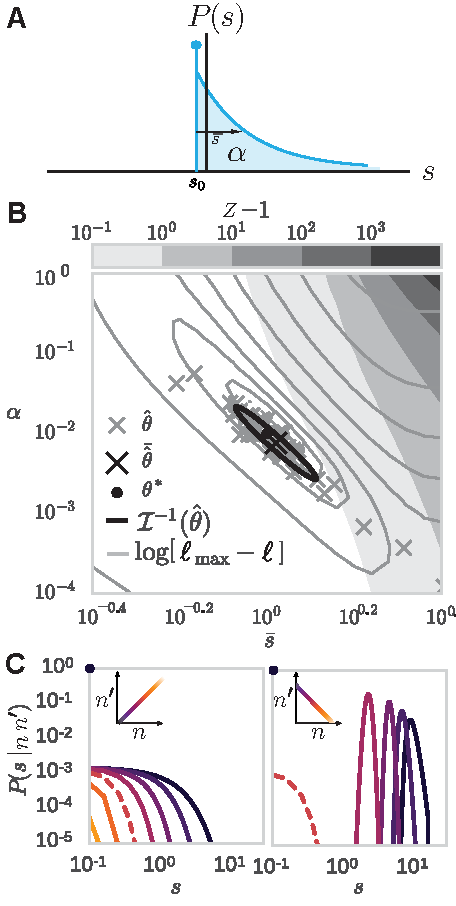
\includegraphics{fig5_diffexpr_eval}
\centering{}
\caption{
\emph{Inference of clonal expansion on synthetic data.}(A) The prior distribution of expansion log fold-changes, $\rho_s(s)$, is parametrized by a mean effect size, $\bar{s}$, describing the expansion of the responding fraction, $\alpha$ of the repertoire  (\cref{eq:onesidedexp}). 
Expansion is relative to a basal $s_0$ fixed by the normalization constraint.
(B) Re-inference of the expansion parameters from synthetic data generated with value $\theta_{\rm exp}^*=(\bar{s}^*,\alpha^* )=(1.0,10^{-2})$ (black dot). 
Maximums of the log-likelihood, $\hat\theta_{\rm exp}$, for 50 realizations (gray crosses), along with their average $\bar{\hat{\theta}}$ (black cross). 
The log-likelihood for one realization is shown over logarithmically-spaced gray contours decreasing from the maximum. 
The inverse Fisher information, $\mathcal{I}^{-1}$, for the same realization is shown as the black-lined ellipse centered at $\bar{\hat{\theta}}$, which provides a lower bound to the variance of our ML estimate. 
The gray scale contours increasing to the upper-right denote $Z^\prime/Z-1$, the excess in the used normalization. (C) Posteriors of the learned model, $\rho(s|n,n^{\prime})$ over pairs $(n,n^{\prime})$ for $n^{\prime}=n$, with $n$ varying over a logarithmically-spaced set of counts (left), and for $n^{\prime}$ given by the reverse order of this set (right). The black dot in both plots denotes the contribution of the non-responding component, $\propto \delta(s-s_0)$, to the posterior.
(Parameters: $N=10^6$, $\epsilon=10^{-2}$.)
\label{fig:diffexpr_ex1}
}
\end{figure}

Note that the value of the true responding fraction $\alpha$ is correctly learned from our procedure, regardless of our ability to tell with perfect certainty which particular clones responded. By contrast, a direct estimate of the responding fraction from the number of significantly responding clones, as determined by differential expression software such as EdgeR \cite{Robinson2010}, is likely to misestimate that fraction. We applied EdgeR to a synthetic repertoire of $N=10^9$ clones, a fraction $\alpha=0.01$ of which responded with mean effect $\bar s=1$, and sampled with $N_{\rm read}=10^6$. EdgeR found $6,880$ significantly responding clones (corrected p-value 0.05) out of $N_{\rm obs}=1,995,139 $, i.e. a responding fraction $6,880/1,995,139 \approx 3\cdot 10^{-3}$ of the observed repertoire, and a responding fraction $6,880/10^9\approx 7\cdot 10^{-6}$ of the total repertoire, underestimating the true fraction $\alpha=10^{-2}$.

\subsection*{Inference of the immune response following immunization} \label{sec:diffexpr}

Next, we ran the inference procedure on sequences obtained from human blood samples across time points following yellow fever vaccination. To guide the choice of prior for $s$, we plotted the histograms of the naive log fold-change $\ln n^{\prime}/n$ (\cref{fig:SM_snaive_hists}). These distributions show symmetric exponential tails, motivating us to model the statistics of expansion factors as:
\beq\label{eq:symmexp}
\rho_{\rm exp}(s)=\frac{1}{2\bar s}e^{-|s|/\bar s},
\eeq
with typical effect size $\bar{s}$.

We applied the inference procedure (Eq.~\ref{eq:MLEexp}) between the repertoires taken the day of vaccination (day 0), and at one of the other time points (day -7, day 7, day 15, and day 45) after vaccination. Since there are two replicates at each time point, we can make 4 comparisons between any pair of time points.

Same-day comparisons (day 0 vs day 0) gave effectively zero mean effect sizes ($\bar s<0.1$, below the discretization step of the integration procedure), as expected (Fig.~\ref{fig:diffexpr_ex2}). Comparisons with other days yielded inferred values of $\alpha$ and $\bar s$ distributed along the same  `ridge' (Fig.~\ref{fig:diffexpr_ex2}), as observed on synthetic data (\cref{fig:diffexpr_ex1}). The mean effect size $\bar s$ is highest at day 15, where the peak of the response occurs, but is also substantially different from 0 at all time points except day 0 (including before vaccination at day $-7$), with often high values of $\alpha$. We speculate that these fluctuations reflect natural variations of the repertoire across time, as well as experimental batch effects. As a consequence of the natural diversity, 
values of the responding fraction $\alpha$ are not learned with great precision, as can be seen from the variability across the 4 choices of replicate pair, and are probably gross overestimations of the true probability that a naive T cell responds to an infection, which is believed to be of order $10^{-5}-10^{-3}$ \cite{Boer1993}.


\begin{figure}
\includegraphics[width=\linewidth]{sbar_alp_vals_linscale}
\centering{}
\caption{
\emph{Application to yellow fever vaccination data.} Optimal values of $\alpha$ and $\bar{s}$ across all 6 donors and days relative to the day of vaccination (day 0). Inset shows the same data on a logarithmic scale for comparison with \cref{fig:diffexpr_ex1}b. Comparisons with days other than 0 fall on straight line (dashed line).
\label{fig:diffexpr_ex2}
}
\end{figure}
